\documentclass[
  bibliography=totoc,     % Literatur im Inhaltsverzeichnis
  captions=tableheading,  % Tabellenüberschriften
  titlepage=firstiscover, % Titelseite ist Deckblatt
]{scrartcl}

% Paket float verbessern
\usepackage{scrhack}

% Warnung, falls nochmal kompiliert werden muss
\usepackage[aux]{rerunfilecheck}

% unverzichtbare Mathe-Befehle
\usepackage{amsmath}
% viele Mathe-Symbole
\usepackage{amssymb}
% Erweiterungen für amsmath
\usepackage{mathtools}

% Fonteinstellungen
\usepackage{fontspec}
% Latin Modern Fonts werden automatisch geladen
% Alternativ:
%\setromanfont{Libertinus Serif}
%\setsansfont{Libertinus Sans}
%\setmonofont{Libertinus Mono}
\recalctypearea % Wenn man andere Schriftarten gesetzt hat,
% sollte man das Seiten-Layout neu berechnen lassen

% deutsche Spracheinstellungen
\usepackage{polyglossia}
\setmainlanguage{german}


\usepackage[
  math-style=ISO,    % ┐
  bold-style=ISO,    % │
  sans-style=italic, % │ ISO-Standard folgen
  nabla=upright,     % │
  partial=upright,   % ┘
  warnings-off={           % ┐
    mathtools-colon,       % │ unnötige Warnungen ausschalten
    mathtools-overbracket, % │
},                       % ┘
]{unicode-math}

% traditionelle Fonts für Mathematik
\setmathfont{Latin Modern Math}
% Alternativ:
%\setmathfont{Libertinus Math}

\setmathfont{XITS Math}[range={scr, bfscr}]
\setmathfont{XITS Math}[range={cal, bfcal}, StylisticSet=1]

% Zahlen und Einheiten
\usepackage[
locale=DE,                   % deutsche Einstellungen
separate-uncertainty=true,   % immer Fehler mit \pm
per-mode=symbol-or-fraction, % / in inline math, fraction in display math
]{siunitx}

% chemische Formeln
\usepackage[
version=4,
math-greek=default, % ┐ mit unicode-math zusammenarbeiten
text-greek=default, % ┘
]{mhchem}

% richtige Anführungszeichen
\usepackage[autostyle]{csquotes}

% schöne Brüche im Text
\usepackage{xfrac}

% Standardplatzierung für Floats einstellen
\usepackage{float}
\floatplacement{figure}{htbp}
\floatplacement{table}{htbp}

% Floats innerhalb einer Section halten
\usepackage[
section, % Floats innerhalb der Section halten
below,   % unterhalb der Section aber auf der selben Seite ist ok
]{placeins}

% Seite drehen für breite Tabellen: landscape Umgebung
\usepackage{pdflscape}

% Captions schöner machen.
\usepackage[
  labelfont=bf,        % Tabelle x: Abbildung y: ist jetzt fett
  font=small,          % Schrift etwas kleiner als Dokument
  width=0.9\textwidth, % maximale Breite einer Caption schmaler
]{caption}
% subfigure, subtable, subref
\usepackage{subcaption}

% Grafiken können eingebunden werden
\usepackage{graphicx}
% größere Variation von Dateinamen möglich
\usepackage{grffile}

% schöne Tabellen
\usepackage{booktabs}

% Verbesserungen am Schriftbild
\usepackage{microtype}

% Literaturverzeichnis
\usepackage[style=alphabetic,]{biblatex}
% Quellendatenbank
\addbibresource{lit.bib}
\addbibresource{programme.bib}

% Hyperlinks im Dokument
\usepackage[
  unicode,        % Unicode in PDF-Attributen erlauben
  pdfusetitle,    % Titel, Autoren und Datum als PDF-Attribute
  pdfcreator={},  % ┐ PDF-Attribute säubern
  pdfproducer={}, % ┘
]{hyperref}
% erweiterte Bookmarks im PDF
\usepackage{bookmark}

% Trennung von Wörtern mit Strichen
\usepackage[shortcuts]{extdash}

\title{V64: Moderne Interferometrie}
\author{
  Simon Schulte
  \texorpdfstring{
    \\
    \href{mailto:simon.schulte@udo.edu}{simon.schulte@udo.edu}
  }{}
  \texorpdfstring{\and}{, }
  Tim Sedlaczek
  \texorpdfstring{
    \\
    \href{mailto:tim.sedlaczek@udo.edu}{tim.sedlaczek@udo.edu}
  }{}
}
\publishers{TU Dortmund – Fakultät Physik}

\date{Durchführung: 13.06.2018\\
      Abgabe: 15.06.2018}


\begin{document}

\maketitle
\thispagestyle{empty}
\setcounter{page}{1}
\pagenumbering{arabic}
\section{Theorie}
\label{sec:theorie}


\section{Auswertung}
\label{sec:auswertung}


\subsection{Fehlerrechnung}
\label{sec:fehlerrechnung}
Für die Fehlerrechnung sowie den mathematischen Teil der Auswertung wird auf
  $\textsc{Python}$ \cite{python} zurückgegriffen:\\
Die in der Auswertung verwendeten Mittelwerte mehrfach gemessener Größen sind
gemäß der Gleichung
\begin{equation}
    \bar{x}=\frac{1}{n}\sum_{i=1}^n x_i.
    \label{eq:mittelwert}
\end{equation}

bestimmt. Dieser ist implementiert durch die Funktion $\textsc{mean}$ aus dem Paket
  $\textsc{Numpy}$ \cite{numpy}. Die Standardabweichung des Mittelwertes ergibt sich dabei zu

\begin{equation}
    \mathup{\Delta}\bar{x}=\sqrt{\frac{1}{n(n-1)}\sum_{i=1}^n\left(x_i-\bar{x}\right)^2}.
    \label{eq:standardabweichung}
\end{equation}

Dieser wird durch die
$\textsc{scipy.stats}$ \cite{scipy} Funktion $\textsc{sem}$ berechnet.\\
Fehlerfortpflanzung wird
durch die Bibliothek $\textsc{uncertainties}$ \cite{uncertainties} automatisiert.
Regressionen sowie deren Fehler wurden durch die $\textsc{Numpy}$
Funktion $\textsc{curve-fit}$ berechnet.
Grafiken wurden mit $\textsc{matplotlib}$ \cite{matplotlib}
erstellt.
\subsection{Kontrastmessung}
Um den Kontrast zu bestimmen werden an einer Photodiode abfallende
Minimal- und Maximalspannungen für verschiedene Polarisatorstellungen
$\theta_{\symup{P}}$ gemessen. Die gemessenen
Werte und die damit errechneten Kontrastwerte nach \eqref{eqn:1} sind in Tabelle \ref{A_tab:1}
zu sehen. Der Kontrast, der abhängig von eingestellten Winkel ist, wird nach
\eqref{eqn:2} mit einer Funktion
\begin{equation}
  K(\theta_{\symup{P}}) = |{\alpha \sin{(\beta \theta_{\symup{P}}+\gamma)}}| + \delta
  \label{A_eqn:1}
\end{equation}
gefittet. Dabei ergeben sich die Parameter:
\begin{align}
\begin{split}
  \alpha &= \num{0.758(3)}\\
  \beta &= \num{1.916(35)}\\
  \gamma &= \SI{-0.087(31)}{\degree} \\
  \delta &= \num{0.007(25)}
\end{split}
\label{A_eqn:2}
\end{align}
Der dazugehörige Fit ist in Abbildung \ref{A_abb:1} dargestellt. Um den Kontrast
optimal unteruschen zu können, wird das Maximum der Kontrastfunktion \eqref{A_eqn:1} gesucht.
Dafür nutzt man die Ableitung und es ergibt sich die notwengdige Bedingung:
\begin{equation*}
  \frac{dK(\theta_{\symup{P}})}{d\theta_{\symup{P}}} = \alpha \beta \cos{
  (\beta \theta_{\symup{P}} + \gamma)} \stackrel{!}{=} 0.
\end{equation*}
Mit Hilfe von
\begin{equation*}
  \beta \theta_{\symup{P, max}} + \gamma = \frac{\pi}{2} \; \leftrightarrow \;
  \theta_{\symup{P, max}} = \frac{\frac{\pi}{2} - \gamma}{\beta}
\end{equation*}
folgt, mit Hilfe der Fitparameter aus \eqref{A_eqn:2} ein Wert von
\begin{equation*}
  \theta_{\symup{P, max}} = \SI{49.6(13)}{\degree}.
\end{equation*}
Die folgenden Messungen wurden bei dieser Polarisatorstellung durchgeführt.
\begin{table}[h!]
  \centering
  \caption{Die Mess- und Kontrastwerte $K$.}
  \label{A_tab:1}
  \begin{tabular}{c c c c}
    \toprule
    $\theta_{\symup{P}}$ / \si{\degree} & $I_{\symup{max}}$ / \si{\volt} &
    $IU_{\symup{min}}$ / \si{\volt} & $K$\\
    \midrule
    0 & -4.31 & -3.72 & 0.07 \\
    10 & -3.62 & -2.31 & 0.22 \\
    20 & -3.22 & -1.28 & 0.43 \\
    30 & -2.94 & -0.72 & 0.61 \\
    35 & -2.92 & -0.67 & 0.63 \\
    40 & -3.08 & -0.53 & 0.70 \\
    45 & -3.23 & -0.47 & 0.75 \\
    50 & -3.56 & -0.41 & 0.80 \\
    55 & -3.88 & -0.50 & 0.77 \\
    60 & -4.28 & -0.75 & 0.70 \\
    70 & -5.03 & -1.06 & 0.65 \\
    80 & -5.25 & -2.19 & 0.41 \\
    90 & -4.84 & -3.72 & 0.13 \\
    \bottomrule
  \end{tabular}
\end{table}

\begin{figure}[h!]
  \centering
  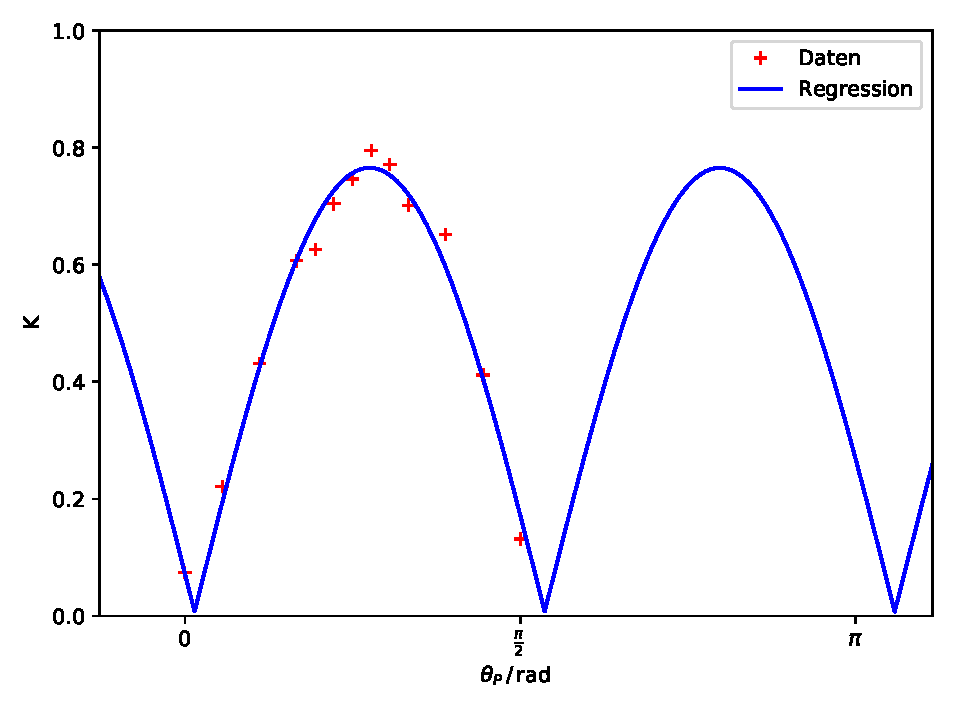
\includegraphics[width=0.7\textwidth]{Kontrast.pdf}
  \caption{Der Kontrast $K$ des Interferometers in Abhängigkeit von der Polarisatorstellung
  $\theta_{\symup{P}}$ mit einer Regression.}
  \label{A_abb:1}
\end{figure}
\noindent
\subsection{Brechungsindex von Glas}
Um einen brauchbaren Zusammenhang zur Bestimmung des Brechungsindex der Glasplättchen
zu erhalten, sind einige Vorüberlegungen notwendig. Die Glasplättchen sind in einem
relativen Winkel $\Theta = 2 \theta_0 = 2 \cdot \SI{10}{\degree}$ zueinander
angeordnet. Gleichung \eqref{T_eq:1} muss daher um
den Winkel $\pm \theta_0$ taylorentwickelt werden. Terme ab $\theta^2$
werden dabei vernachlässigt. Es ergibt sich:
\begin{gather*}
  \mathcal{T}_{(1)}M(\theta,\theta_0) = \frac{T}{\lambda}\cdot\frac{n-1}{2n}(\theta_0^2 + 2\theta_0(\theta-\theta_0)),\\
  \mathcal{T}_{(1)}M(\theta,-\theta_0) = \frac{T}{\lambda}\cdot\frac{n-1}{2n}(\theta_0^2 - 2\theta_0(\theta+\theta_0)).
\end{gather*}
Um einen Zusammenhang für den Brechungsindex des Scheibenmaterials zu erhalten, muss
die Differenz der beiden Entwicklungen gebildet werden. Umgestellt nach $n$ folgt:
\begin{equation}
  n = \left( 1 - \frac{\lambda{M}}{2T\theta_0\theta} \right)^{-1}.
\label{A_eqn:3}
\end{equation}
Die mit \eqref{A_eqn:3} und einer Plättchendicke von $T=\SI{1}{\milli\metre}$
sowie einer Laserwellenlänge von \SI{633}{\nano\metre}
aus den Messdaten erhaltenen Werte finden sich in Tabelle
\ref{A_tab:2}, wobei $\theta_0 = \SI{10}{\degree}$ gilt. Es wurden 5 Messreihen
aufgenommen. Mittelung über die Messwerte aller Messreihen liefert einen Wert von:
\begin{equation*}
  n_{\symup{Glas}} = \num{1.561(12)}.
\end{equation*}

\begin{table}[h!]
  \centering
  \caption{Messwerte mit Brechungsindizes der 5 Messreihen. Es wurde ein
  Intervall von \SI{10}{\degree} abgefahren.}
  \label{A_tab:2}
  \begin{tabular}{c | c}
    \toprule
    $M$ & $n$ \\
    \midrule
    34 & 1.60 \\
    34 & 1.55 \\
    35 & 1.57 \\
    35 & 1.57 \\
    35 & 1.52 \\
    \bottomrule
  \end{tabular}
\end{table}

\subsection{Brechungsindex von Luft}
Messwerte und nach \eqref{T_eq:2} bestimmte Brechungsindizes sind in Tabelle
\ref{A_tab:3} dargestellt. Alle Interfernzstreifenmessungen wurden mit einem Fehler
von $\pm \, 2$ versehen, da es bei der Rückkehr auf Umgebungsdruck in der Gaszelle
zu Fehlzählungen kommt. Die Länge der Zelle beläuft sich auf $L = \SI{10}{\centi\metre}$.
Wieder beträgt die Laserwellenlänge \SI{633}{\nano\metre}.\\
Es ergibt sich also ein Wert von
\begin{equation*}
  n_{\symup{Luft}} = \num{1.000268(13)}.
\end{equation*}

\begin{table}[h!]
  \centering
  \caption{Gezählte Interferenzstreifen $M$ mit berechneten
  Brechungsindizes für Luft und Mittelwert $\overline{n}$.}
  \label{A_tab:3}
  \begin{tabular}{c c c}
    \toprule
    & $M$ & $n$ \\
    \midrule
    & 43 $\pm$ 2 & \num{1.000272(13)} \\
    & 42 $\pm$ 2 & \num{1.000266(13)} \\
    & 42 $\pm$ 2 & \num{1.000266(13)} \\
    \midrule
    $\overline{n}$ & & \num{1.000268(13)}\\
    \bottomrule
  \end{tabular}
\end{table}

\section{Diskussion}
\begin{table}[h!]
  \centering
  \caption{Übersicht über die Messergebnisse mit Literaturwerten.}
  \label{D_tab:1}
  \begin{tabular}{c c c}
    \toprule
    & Messung & Literatur \\
    \midrule
    $n_{\symup{Glas}}$ & \num{1.561(12)} & \num{1.5} \cite[S. 11-5]{anleitung}  \\
    $n_{\symup{Luft, \SI{633}{\nano\metre}}}$ & \num{1.000268(13)} & \num{1.000277} \cite{Luft} \\
    \bottomrule
  \end{tabular}
\end{table}

Tabelle \ref{D_tab:1} beinhaltet die gemessenen und die Literaturwerte. Es zeigt sich, dass
der Literaturwert für die Luftmessung in der Messungenauigkeit liegt.
Der in dem Versuch errechnete Wert für die Glasmessunghat allerdings nur eine
sehr kleine Abweichung zum Literaturwert. Das könnte eventuell an dem verwendeten
Glas liegen. Dies könnte eine andere Zusammensetzung haben, als das, das für den Literaturwert
genutzt wurde.
Bei der Messung des Brechnungsindex' von Luft konnte das Fehlerintervall nur getroffen
werden, da die Interfernzstreifenzählung nicht als fehlerfrei angesehen werden konnte
und ein pauschaler Fehler von $\pm \,\, 2$ angenommen wurde.
Es konnte außerdem beobachet werden, dass manchmal die Interferenzstreifen
von der Ausleseelektronik nicht aufgenommen werden konnten, da der Druck in der
Gaszelle etwas zu rasant anstieg. Daher ist hier ein systematischer
Fehler nicht auszuschließen. Dennoch ist der errechnete Wert ziemlich präzise am
Literaturwert.\\
Als weitere Fehlerquelle ergibt sich auch die Justage des Interferometers.
Bei der Kontrastfunktion zeigt sich eine relativ eindeutige $\frac{\pi}{2}$-Periode
und auch das Maximum ist in dem zu erwarteten Bereich. Allerdings sind auch
Fehler sichtbar, die durch eine bessere Justage verbessert werden könnten.
Dadurch würde sich ein besserer Kontrastwert ergeben und damit wäre das Auflösungsvermögen
des Interferometers besser.


\newpage
\nocite{*}
\printbibliography
\end{document}
